% This work is licensed under the Creative Commons Attribution-NonCommercial 4.0 International License.
% To view a copy of this license, visit http://creativecommons.org/licenses/by-nc/4.0/
% or send a letter to Creative Commons, PO Box 1866, Mountain View, CA 94042, USA.

% !TEX TS-program = xelatex

\documentclass[../Main/notes.tex]{subfiles}

\setcounter{chapter}{7}
\begin{document}

\chapter{Geometry optimization and transition state search}

In this chapter we discuss some of the basic aspects of algorithms for geometry optimization.
We will also take a look at the problem of finding transition states.

\section{Geometry optimization algorithms}
The main goal of geometry optimization algorithms is to find stationary points on a PES.
Recall that at a stationary point the gradient of the energy with respect to coordinate $R_i$, which we indicate with $g_i$, is equal to zero
\begin{equation}
g_i = \left.\frac{\partial E(\mathbf{R})}{\partial R_i}\right|_{\mathbf{R}=\mathbf{R}^*} = 0, i=1,\ldots,3 N_\mathrm{atoms}
\end{equation}
This expression refers to all the $3 N_\mathrm{atoms}$ \emph{Cartesian coordinates}, which means that the$R_i$ stands for any of the $X$, $Y$, or $Z$ coordinates of the atoms.

How do geometry optimization algorithms find stationary points?
Consider the potential energy curve of a diatomic molecule, $E(r)$ , which depends on the bond distance $r$.
Suppose that we have guessed that the bond length is going to be close to some value $r_0$.
In the previous section we have seen that $E(r)$ can be approximated by a Taylor series as
\begin{equation}
\begin{split}
E(r) & = E(r_0) + E'(r_0) (r - r_0) + \frac{1}{2} E''(r_0) (r - r_0)^2 + \ldots \\
& = E(r_0) + g (r - r_0) + \frac{1}{2} h (r - r_0)^2 + \ldots
\end{split}
\end{equation}
where $g = E'(r_0)$ and $h = E''(r_0)$ are the gradient and hessian, respectively.
Note that in this case we \emph{are not at a stationary point}, so the gradient will not be zero, $g \neq 0$.

How can get closer to the stationary point?
One of the simplest algorithms is the \emph{Newton--Raphson method} (NR).
Remember that at a stationary point $r^*$, the energy satisfies the condition $E'(r^*) = 0$. This suggests that we can try to find the value of $r$ such that the first derivative of the \emph{Taylor approximation} is equal to zero.
If we take the derivative of the Taylor series of $E(r)$ we get
\begin{equation}
E'(r)  = g + h (r - r_0) + \ldots 
\end{equation}
If we impose on this expression the condition $E'(r^*) = 0$ and ignore the quadratic terms and higher ($\ldots$), we obtain the condition
\begin{equation}
g + h ( r^* - r_0) = 0 \quad \Rightarrow 
\quad 
r^* = r_0 - \frac{g}{h}
\end{equation}
This equation tells us at what bond distance we will find the stationary point, \emph{if the potential energy curve is quadratic}. In practice, the potential contains terms beyond quadratic, but if we are close enough to a stationary point they will only amount to a small correction.
In this case we can repeat the Newton--Raphson procedure and recompute the gradients and hessians and continue to update the geometry until the gradient is close enough to zero.
As we get closer to the stationary point, cubic and higher terms in the Taylor expansion become smaller, and the Newton--Raphson procedure predicts a more geometry.

For a polyatomic molecule, this procedure can be easily generalized and it leads to the following rule to update the geometry
\begin{equation}
R_i = R_{0,i} - \sum_{j}^{3 N_\mathrm{atoms}}(H^{-1})_{ij} g_j
\end{equation}
where $(H^{-1})_{ij}$ is the inverse Hessian matrix, while $R_i$ and $R_{0,i}$ are the new and old values of the $i$-th coordinate, respectively.

Convergence of the energy optimization is determined by monitoring several variables.
\begin{myitems}
\item The energy change after one step in the optimization, $\Delta E = E(\mathbf{R}) - E(\mathbf{R}_0)$.
\item The maximum force (the maximum value of $g_i$) and the root mean square (RMS) force, $\sqrt{\frac{1}{3 N_\mathrm{atoms}}\sum_i g_i^2}$.
\item The maximum displacement (the maximum value of $R_i - R_{0,i}$) and the RMS deviation, $\sqrt{\frac{1}{3 N_\mathrm{atoms}}\sum_i (R_i - R_{0,i})^2}$.
\end{myitems}
The reason for using all these metrics is that we want to guarantee that both the energy and geometry are well optimized.
In certain case, for example, when the potential energy surface is nearly flat, the optimization steps only produce small changes in the energy but large displacements.
In this case monitoring only the energy would prematurely stop the optimization.

Note that other optimization algorithms exist.
When analytic energy gradients are not available, it is possible to optimize the energy using \emph{derivative-free algorithms} like the Nelder--Mead method.
Algorithms like \emph{gradient descent} optimize the geometry along the direction of the gradient, but determine the step without the Hessian.

\section{Analytical vs. numerical gradients and choice of the Hessian}
Molecular optimization are most easily performed when the gradient can be computed by direct differentiation of the energy.
For example consider the function $f(x) = \exp(-x^2)$.
We can immediately compute the \emph{analytic gradient} of $f(x)$ by applying the rules of calculus
\begin{equation}
f\,'(x) = -2 x \exp(-x^2)
\end{equation}
However, suppose we did not know how to take the derivative of $\exp$ or powers of $x$. In this case we can always apply the definition of the derivative
\begin{equation}
f\,'(x) = \lim_{h \rightarrow 0} \frac{f(x + h) - f(x)}{h}
\end{equation}
Since we cannot compute the limit numerically, we can always approximate it by \emph{finite difference}, that is, by using a small value of $h$
\begin{equation}
f\,'(x) \approx \frac{f(x + h) - f(x)}{h} + \text{error of order } h
\end{equation}
The error we make using this formula is proportional to $h$, so if we make $h$ sufficiently enough\mnote{Here $h$ must be still large enough to avoid rounding errors.} we can produce an accurate approximation to $f\,'(x)$.\mnote{There are better formulas for approximating the first derivative. For example, the 
$$
f\,'(x) \approx \frac{f(x + h) - f(x-h)}{2h}
$$
introduces an error proportional to $h^2$, so if we use $h= 0.001$, the error will be of the order of $10^{-6}$.
}
Analytic gradients are always preferred because one evaluation of the gradients costs a bit more than a single energy computation.
Obtaining energy gradients via finite difference can be very expensive, because we need to evaluate the energy one or more times for each  coordinate we optimize. This means that the relative cost of computing a gradient grows with the size of a molecule, and it is about 3$N_\mathrm{atoms}$ that of a single energy computation.

Because computing the Hessian is quite expensive, geometry optimization often employs approximate or empirical Hessians.
If a Hessian is not available---which is typically the default assumption of quantum chemistry codes---one may use an empirical hessian based on a `ball-and-sticks' description of atoms in a molecule.
If the Hessian of the initial geometry is available, this may be used to speed up the convergence of a geometry optimization, especially more challenging cases where empirical Hessians are incorrect.
Programs may update the Hessian during the optimization process, or give the option to recompute the Hessian at each step (which is very expensive).
Some times a good option is to start a geometry optimization with an Hessian computed at a very low level of theory.
Since the Hessian provides information about the curvature of the PES, just getting a qualitatively accurate Hessian can be enough to improve the convergence in troubles cases and transition state searches.

\section{Choice of coordinates}

\mfigure{
\centering{
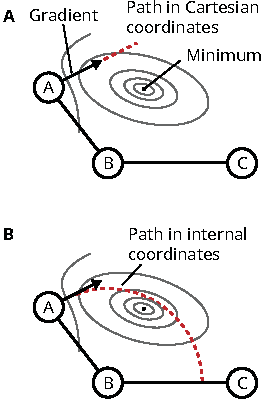
\includegraphics[width=1.75in]{img/coords.pdf}
}
\captionof{figure}{Comparison of optimization of the coordinates of atom A in the triatomic A-B-C in Cartesian (\textbf{A}) and internal coordinates (\textbf{B}). The red line shows the path in which the atom A can move in the two coordinate systems.}
\label{fig:5:coords}
}

Geometry optimization using Cartesian coordinates is not the only possible choice.
Any set of coordinates that fully span the same degrees of freedom of Cartesian coordinates (3$N_\mathrm{atoms}$, linearly independent) may be used to perform a geometry optimization.

In particular, coordinates based on the bond distances and angles offer a very natural way to optimize the geometry of molecules.
Some examples of internal coordinates are interatomic distances, angles, out-of-plane angles, and torsion angles.
For example, \emph{interatomic distance} between atoms A-B ($r_{\mathrm{AB}}$) is defined in terms of the Cartesian positions of atoms A and B [$\mathbf{r}_{A} = (x_\mathrm{A},y_\mathrm{A},z_\mathrm{A})$]
\begin{equation}
r_{\mathrm{AB}} =
\sqrt{
(x_\mathrm{A} - x_\mathrm{B})^2
+ (y_\mathrm{A} - y_\mathrm{B})^2
+ (z_\mathrm{A} - z_\mathrm{B})^2
}
= |\mathbf{r}_{\mathrm{AB}}|
\end{equation}
where $\mathbf{r}_{AB} = \mathbf{r}_{A} - \mathbf{r}_{B}$.
Similarly, the \emph{angle} between atoms A-B-C ($\theta_{\mathrm{ABC}}$) is defined as the angle between the vectors $\mathbf{r}_{AB} = \mathbf{r}_{A} - \mathbf{r}_{B}$ and $\mathbf{r}_{CB} = \mathbf{r}_{C} - \mathbf{r}_{B}$
\begin{equation}
\cos \theta_{\mathrm{ABC}}
= \frac{\mathbf{r}_{AB} \cdot \mathbf{r}_{CB}}
{|\mathbf{r}_{AB}||\mathbf{r}_{CB}|}
\end{equation}
Optimization in internal coordinates requires the generation of a complete set of internal coordinates.
Most codes employ \emph{redundant internal coordinates} by including more coordinates than the number strictly needed.
Redundant internal coordinates lead to faster convergence to stationary points, especially for more challenging systems with cyclic structure.

What is the advantage of using internal coordinates? As shown in Fig.~\ref{fig:5:coords}, internal coordinates allow to step into  curvilinear directions, which sometimes may offer a more rapid convergence.
In this example, the gradient is the same, but the step taken by the optimizer is different depending on the coordinate system used.
In Cartesian coordinates, atom A is displaced along a linear path that follows the direction of the gradient. This path brings the atom closer to the minimum, but it is not optimal.
In contrast, when working internal coordinates, atom A follows a curvilinear path that corresponds to changing the angle A-B-C while keeping the distance A-B fixed.
Stepping along this curved path can bring atom A closer to the minimum.

In which case it is convenient to use Cartesian coordinates?
One example where internal coordinates may fail is when optimizing the structure of weakly interacting molecules.
Since typical implementations automatically generate a set of internals, restricting the coordinates to atoms that are not too far apart, there might not be an internal coordinate that directly controls the distance or orientation between two molecules.
When this happens, an optimization algorithm may take a long time to optimize a molecule.
Cartesian coordinates work better in this case.
It is also possible to mix Cartesian and internal coordinates.
This set of coordinates can lead to more robust optimizations.

\section{Potential energy scans and constrained optimization}

We are often interested in mapping out the energy of a molecule as its geometry changes.
In this case one often performs a series of energy computations in which a small set of geometric parameters (Cartesian or internal) is varied over a range.
This type of computation is called a \emph{potential energy scan}.
Potential energy scans are often used to compute bond dissociation curves, to compute the intermolecular interaction energy between two molecules, or to study how the energy changes as a function of a change in conformation.

A straightforward potential energy scan of polyatomic molecules yields unrelaxed energies, by which we mean that the value of the coordinates that are kept fixed are not optimal.
However, it is possible to relax all other coordinates during a scan with a \emph{constrained optimization}.
For example, suppose you are interested in computing the energy of hydrogen peroxide (HOOH) as a function of the H-O-O-H dihedral angle $\tau$ using the values 0, 5, 10, \ldots, 180\textdegree.
As the dihedral angle changes, the optimal value of the O-H and O-O bond distances and the H-O-O angle will vary, so they need to be optimized.
In a \emph{relaxed potential energy scan} you would loop over each value of $\tau$, and for a given $\tau$  perform an optimization of all other coordinates while keeping the dihedral fixed.
Figure~\ref{fig:5:hooh_rot} shows the result of a scan of the H-O-O-H dihedral angle using relaxed and unrelaxed geometries.
These energies are identical at the value of $\tau$ that minimize the energy, but they differ for smaller and larger values of $\tau$.
Most importantly, the unrelaxed energy is higher than the relaxed one, and the difference is as large as 1 kcal/mol when $\tau = 0$. 

\mfigure{
\centering{
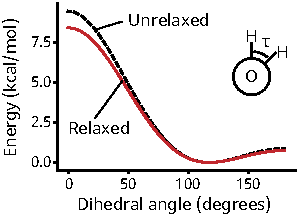
\includegraphics[width=2.00in]{img/hooh_rot.pdf}
}
\captionof{figure}{Hydrogen peroxide (HOOH). Potential energy scan as a function of the dihedral angle $\phi$. The relaxed curve is obtained by constraining the dihedral angle and optimizing all other coordinates. The unrelaxed curve is obtained by fixing the O-H and O-O bond lengths and the H-O-O bond angle at value that correspond to the minimum energy geometry.}
\label{fig:5:hooh_rot}
}

\section{Transition state searches}

Searching for a transition state (TS) is significantly more different than finding minima on the PES.
There are several reasons that make transition state searches more difficult. Transition states are often significantly different than equilibrium molecular geometries and so are difficult to guess. There can also be multiple transition states that connect reactants to products making the search for the lowest energy transition state more difficult.

The easies way to find a transition state is to have a very good guess of what its geometry looks like!
This might be easy for computing the barrier to rotation in a molecule, or for simple reactions like SN$_2$.
When a geometry is sufficiently close to a transition state, and the Hessian has one negative eigenvalue that is well aligned with the reaction coordinate, then the Newton--Raphson method is likely to find the transition state.
This is the case because we did not make assumption regarding the nature of the stationary point in the NR method.
This approach to finding transition states is called a \emph{local search}.
It is mandatory in this case to compute an exact Hessian before performing the transition state search, because if the Hessian comes from a guess that incorrectly assumes all eigenvalues are positive, then the NR method could go in the direction of a minimum.

For relatively simple molecules, transition states may be found by performing a PES scan.
For example, the scan shown in Fig.~\ref{fig:5:hooh_rot} has two transitions states, that connect two minima on the potential energy surface of HOOH (approximately at $\pm 110$\textdegree).
For certain reactions (e.g., SN$_2$), one may be able to find the transition state via a scan of the energy as a function of one of the bond lengths.

\emph{Semi-global} methods are more sophisticated transition state search algorithms that require the user to input a structure for the reactant and optionally that of the product.
Some algorithms are open-ended, meaning that they explore the PES in search of a neaby transition state.
Algorithms that use both the reactant and product geometry try to identify a path that connects these two structures and contains the transition state.
There are a myriad of methods to find transitions states and the best way to learn how to use them is to read the details of the implementation in the manual of the computational program you plan to use.

\section{Intrinsic reaction coordinate (IRC)}

Once you have identified a transition state how do you know that it is the correct one?
An intrinsic reaction coordinate is a path that starts at a transition state and has backward  and forward branches that connect to minima.
By computing the IRC, it is possible to verify that the transition state connects the reactant and product that we are studying.

The IRC is a path in coordinate space $\mathbf{R}(s)$ parameterized by the variable $s$.
This path satisfies the steepest descent differential equation
\begin{equation}
\frac{ d \mathbf{R}(s) }{ d s} = - \frac{\mathbf{g}(s)}{|\mathbf{g}(s)|}
\end{equation}
where $\mathbf{g}(s)$ is the gradient vector at the geometry $\mathbf{R}(s)$.
Therefore, computing the IRC requires only the energy gradient.

Unfortunately there is not a unique way to defined the IRC, and the path you obtain depends on the set of coordinates used by the optimization algorithm.
However, if you plan on doing an IRC computation to verify that you have found a transition state that connects the correct reactant and products, the differences in IRC path will not matter.

\begin{summary}
\item The most efficient geometry optimization algorithms are based on the Newton--Raphson method. They employ both the gradient and Hessian of the energy.
\item Different coordinate sets may be used to perform the optimization. Internal coordinates perform better than Cartesian coordinates in most situations.
\item Potential energy scans may be used to study the energy as a function of a geometric variable.
\item Transition state algorithm are not black-box methods. Most of the time a successful TS search starts from a geometry that is very close to a transition state.
An intrinsic reaction coordinate computation can be used to verify that a transition state connects to the correct reactant and product.
\end{summary}


\end{document}
